% Template for PLoS
% Version 1.0 January 2009
%
% To compile to pdf, run:
% latex plos.template
% bibtex plos.template
% latex plos.template
% latex plos.template
% dvipdf plos.template
\documentclass[11pt]{article}
%\usepackage{natbib}
\usepackage{hyperref}
\usepackage{lineno}

% amsmath package, useful for mathematical formulas
\usepackage{amsmath}
% amssymb package, useful for mathematical symbols
\usepackage{amssymb}
\usepackage{chngpage}
% graphicx package, useful for including eps and pdf graphics
% include graphics with the command \includegraphics
\usepackage{graphicx}

% cite package, to clean up citations in the main text. Do not remove.
\usepackage{cite}

\usepackage{color} 

% Use doublespacing - comment out for single spacing
%\usepackage{setspace} 
%\doublespacing
\newcommand{\peer}{\textit{P. eremicus}} 

% Text layout
\topmargin 0.0cm
\oddsidemargin 0.5cm
\evensidemargin 0.5cm
\textwidth 16cm 
\textheight 21cm
\linespread{1.2}
% Bold the 'Figure #' in the caption and separate it with a period
% Captions will be left justified
\usepackage[labelfont=bf,labelsep=period,justification=raggedright]{caption}

% Use the PLoS provided bibtex style
\bibliographystyle{plos2009}

% Remove brackets from numbering in List of References
\makeatletter
\renewcommand{\@biblabel}[1]{\quad#1.}
\makeatother


% Leave date blank
\date{}

\pagestyle{myheadings}
%% ** EDIT HERE **


%% ** EDIT HERE **
%% PLEASE INCLUDE ALL MACROS BELOW

%% END MACROS SECTION

\begin{document}

% Title must be 150 characters or less
\begin{flushleft}
{\Large
\textbf{Characterization of the transcriptome, nucleotide sequence polymorphism, and natural selection in the desert adapted mouse \textit{Peromyscus eremicus}}
}
% Insert Author names, affiliations and corresponding author email.
\\
Matthew D. MacManes$^{1}$, 
Michael B. Eisen $^{2}$, 
\\
$^{1}$ Department of Molecular, Cellular and Biomedical Sciences, University of New Hampshire, Durham NH, USA
\\
$^{2}$ HHMI and University of California, Berkeley, Berkeley, CA, USA
\\
$\ast$ E-mail: macmanes@gmail.com, @PeroMHC
\end{flushleft}

\linenumbers

% Please keep the abstract between 250 and 300 words
\section*{Abstract}

As a direct result of intense heat and aridity, deserts are thought to be among the most harsh of environments, particularly for their mammalian inhabitants. Given that osmoregulation can be challenging for these animals, with failure resulting in death, strong selection should be observed on genes related to the maintenance of water and solute balance. One such animal, \textit{Peromyscus eremicus}, is native to the desert regions of the southwest United States and may live its entire life without oral fluid intake. As a first step toward understanding the genetics that underlie this phenotype, we present a characterization of the \peer\: transcriptome. We assay four tissues (kidney, liver, brain, testes) from a single individual and supplement this with population level renal transcriptome sequencing from 15 additional animals. We identified a set of transcripts undergoing both purifying and balancing selection based on estimates of Tajima's D. In addition, we used the branch-site test to identify a transcript -Slc2a9, likely related to desert osmoregulation -- undergoing enhanced selection in \peer\: relative to a set of related non-desert rodents.  \\


\section*{Introduction}

Deserts are widely considered one of the harshest environments on Earth. Animals living in desert environments are forced to endure intense heat and drought, and as a result, species living in these environments are likely to posses specialized mechanisms to deal with them. While living in deserts likely involves a large number of adaptive traits, the ability to osmoregulate -- to maintain the proper water and electrolyte balance -- appears to be paramount \cite{Walsberg:2000uu}. Indeed, the maintenance of water balance is one of the most important physiologic processes for all organisms, whether they be desert inhabitants or not. Most animals are exquisitely sensitive to changes in osmolality, with slight derangement eliciting physiologic compromise.  When the loss of water exceeds dietary intake, dehydration - and in extreme cases, death - can occur. Thus there has likely been strong selection for mechanisms supporting optimal osmoregulation in species that live where water is limited. Understanding these mechanisms will significantly enhance our understanding of the physiologic processes underlying osmoregulation in extreme environments, which will have implications for studies of human health, conservation, and climate change. \\

The genes and structures responsible for the maintenance of water and electrolyte balance are well characterized in model organisms such as mice \cite{Tatum:2009kp}, rats \cite{Romero:2007fs,Rojek:2006dg,NIELSEN:1995uq}, and humans \cite{Mobasheri:2007tt,Bedford:2003wa,NIELSEN:1999vg}. These studies, many of which have been enabled by newer sequencing technologies, provide a foundation for studies of renal genomics in non-model organisms. Because researchers have long been interested in desert adaptation, a number of studies have looked at the morphology or expression of single genes in the renal tissues of desert adapted rodents \textit{Phyllotis darwini} \cite{Gallardo:2005fm}, \textit{Psammomys obesus} \cite{Kaissling:1975uu}, and \textit{Perognathus penicillatus} \cite{Altschuler:1979du}. More recently, full renal transcriptomes have been generated for \textit{Dipodomys spectabilis} and \textit{Chaetodipus baileyi}, \cite{Marra:2014de} as well as \textit{Abrothrix olivacea} \cite{Giorello:2014iv}. \\

These studies provide a rich context for current and future work aimed at developing a synthetic understanding of the genetic and genomic underpinnings of desert adaptation in rodents. As a first step, we have sequenced, assembled, and characterized the transcriptome (using four tissue types - liver, kidney, testes and brain) of a desert adapted cricetid rodent endemic to the southwest United States \cite{Veal:2001vp}, \textit{Peromyscus eremicus}. These animals have a lifespan typical of small mammals, and therefore an individual may live its entire life without ever drinking water. These rodents have distinct advantage over other desert animals (e.g. \textit{Dipodomys}) in that they breed readily in captivity, which enables future laboratory studies of the phenotype of interest. In addition, the focal species is positioned in a clade of well known animals (e.g. \textit{P. californicus}, \textit{P. maniculatus}, and \textit{P. polionotus}) \cite{Bradley:2007jo} with growing genetic and genomic resources \cite{Shorter:2014kw,Panhuis:2011co,Shorter:2012ib}. Together, this suggests that future comparative studies are possible. \\

While the elucidation of the mechanisms underlying adaptation to desert survival is beyond the scope of this manuscript, we aim to lay the groundwork by characterizing the transcriptome from four distinct tissues (brain, liver, kidney, testes). These data will be included in the current larger effort aimed at sequencing the entire genome. Further, via sequencing the renal tissue of a total of 15 additional animals, we characterize nucleotide polymorphism and genome-wide patterns of natural selection. Together, these investigations will aid in our overarching goal to understand the genetic basis of adaptation to deserts in \textit{P. eremicus}.

\section*{Materials and Methods}

\subsection*{Animal Collection and Study Design}

To begin to understand how genes may underlie desert adaptation, we collected 16 individuals from a single population of \textit{P. eremicus} over a two-year time period (2012-2013). These individuals were captured in live traps and then euthanized using isoflurane overdose and decapitation. Immediately post-mortem, the abdominal and pelvic organs were removed, cut in half (in the case of the kidneys), placed in RNAlater and flash frozen in liquid Nitrogen. Removal of the brain, with similar preservation techniques, followed. Time from euthanasia to removal of all organs never exceeded five minutes. Samples were transferred to a -80C freezer at a later date. These procedures were approved by the Animal Care and Use Committee located at the University of California Berkeley (protocol number R224) and University of New Hampshire (protocol number 130902) as well as the California Department of Fish and Game (protocol SC-008135) and followed guidelines established by the American Society of Mammalogy for the use of wild animals in research \cite{Sikes:2011dz}.  

\subsection*{RNA extraction and Sequencing}

Total RNA was extracted from each tissue using a TRIzol extraction (Invitrogen) following the manufacturer's instructions. Because preparation of an RNA library suitable for sequencing is dependent on having high
quality, intact RNA, a small aliquot of each total RNA extract was
analyzed on a Bioanalyzer 2100 (Agilent, Palo Alto, CA, USA).
Following confirmation of sample quality, the reference sequencing libraries
were made using the TruSeq stranded RNA prep kit
(Illumina), while an unstranded TruSeq kit was used to construct the other sequencing libraries. A unique index was ligated to each sample to allow for multiplexed sequencing. Reference libraries (n=4 tissue types) were then pooled to
contain equimolar quantities of each individual library and
submitted for Illumina sequencing using two lanes of 150nt paired end sequencing employing the rapid-mode of the HiSeq 2500 sequencer at The Hubbard Center for Genome Sciences (University of New Hampshire). The remaining 15 libraries were similarly multiplexed and sequenced in a mixture of 100nt paired and single end sequencing runs across several lanes of an Illumina HiSeq 2000 at the Vincent G. Coates Genome Center (University of California, Berkeley).

\subsection*{Sequence Data Preprocessing and Assembly}

The raw sequence reads corresponding to the four tissue types were error corrected using the software bless \cite{Heo:2014cb} using kmer=25, based on the developer's default recommendations. The error-corrected sequence reads were adapter and quality trimmed following recommendations from MacManes \cite{MacManes:2014io} and Mbandi \cite{Christoffels:2014bg}. Specifically, adapter sequence contamination and low quality nucleotides (defined as \textsc{Phred} \textless 2) were removed using the program Trimmomatic version 0.32  \cite{Lohse:2012fg}. Reads from each tissue were assembled using the Trinity version released 17 July 2014 \cite{Haas:2013jq}. We used flags to indicate the stranded nature of sequencing reads and set the maximum allowable physical distance between read pairs to 999nt. The assembly was conducted on a linux workstation with 64 cores and 512Gb RAM. To filter the raw sequence assembly, we downloaded \textit{Mus musculus} cDNA and ncRNA datasets from Ensembl (\url{ftp://ftp.ensembl.org/pub/release-75/fasta/mus_musculus/}) and the \textit{Peromyscus maniculatus} reference transcriptome from NCBI (\url{ftp://ftp.ncbi.nlm.nih.gov/genomes/Peromyscus_maniculatus_bairdii/RNA/}). We used a blastN procedure (default settings, evalue set to 10$^{-10}$) to identify contigs in the \textit{P. eremicus} dataset likely to be biological in origin. This procedure, when a reference dataset is available, retains more putative transcripts that a strategy employing expression-based filtering (remove if TMP \textless 1  \cite{MacManes:2012bu}) of the raw assembly. We then concatenated the filtered assemblies from each tissue into a single file and reduced redundancy using the software cd-hit-est \cite{Li:2006hr} using default setting, except that sequences were clustered based on 95\% sequence similarity. This multi-fasta file was used for all subsequent analyses, including annotation and mapping. \\

\subsection*{Assembled Sequence Annotation}



The filtered assemblies were annotated using the default settings of the blastN algorithm \cite{Camacho:2009fc} against the Ensembl cDNA and ncRNA datasets described above, downloaded on 1 August 2014. Among other things, the Ensemble transcript identifiers were used in the analysis of gene ontology conducted in the PANTHER package \cite{Mi:2004iv}. Next, because rapidly evolving nucleotide sequences may evade detection by blast algorithms, we used HMMER3 \cite{Wheeler:2013gj} to search for conserved protein domains contained in the dataset using the Pfam database \cite{Punta:2012ko}. Lastly, we extracted putative coding sequences using Transdecoder version 4Jul2014 (\url{http://transdecoder.sourceforge.net/})\\

To identify patterns of gene expression unique to each tissue type, we mapped sequence reads from each tissue type to the reference assembly using bwa-mem \cite{Li:2013wn}. We estimated expression for the four tissues individually using default settings of the software eXpress \cite{Roberts:2012dh}. Interesting patterns of expression, including instances where expression was limited to a single tissue type, were identified and visualized. \\ 

\subsection*{Population Genomics}

In addition to the reference individual sequenced at four different tissue types, we sequenced 15 other conspecific individuals from the same population in Palm Desert, California. Sequence data were mapped to the reference transcriptome using bwa-mem. The alignments were sorted and converted to BAM format, then passed to the program \textsc{Angsd} version 0.610, which was used for calculating the folded site frequency spectrum (SFS) and Tajima's D \cite{Korneliussen:2013uz}. \\


\subsection*{Natural Selection}

To characterize natural selection on several genes related to water and ion homeostasis, we identified several of the transcripts identified as experiencing positive selection in a recent work on desert-adapter \textit{Dipodomys} rodents. The coding sequences corresponding to these genes, Solute Carrier family 2 member 9  (Slc2a9) and the Vitamin D3 receptor (Vdr), were extracted from the dataset, aligned using the software MACSE \cite{Ranwez:2011kj} to homologous sequences in \textit{Mus musculus}, \textit{Rattus norvegicus}, \textit{Peromyscus maniculatus}, and \textit{Homo sapiens} as identified by the conditional reciprocal best blast procedure (CRBB, \cite{Aubry:2014en}). An unrooted gene tree was constructed using the online resource Clustal-Omega, and the tree and alignment were analyzed using the branch-site model (model=2, nsSites=2, fix\_omega=0 versus model=2, nsSites=2, fix\_omega=1, omega=1)  implemented in PAML version 4.8 \cite{Yang:2011bm,Yang:2007ki}. Significance was evaluated via the use of the likelihood ratio test. \\   


% Results and Discussion can be combined.
\section*{Results and Discussion}

\subsection*{RNA extraction, Sequencing, Assembly, Mapping}

RNA was extracted from the hypothalamus, renal medulla, testes, and liver from each individual using sterile technique. TRIzol extraction resulted in a large amount of high quality (RIN $\geq$ 8) total RNA, which was then used as input. Libraries were constructed as per the standard Illumina protocol and sequenced as described above. The number of reads per library varied from 56 million strand-specific paired-end reads in Peer360 kidney, to 9 million single-end reads in Peer321 (\hypertarget{Table 1}{Table 1}, available on the Short Read Archive accession XXX). Adapter sequence contamination and low-quality nucleotides were eliminated, which resulted in a loss of \textless 2\% of the total number of reads. These trimmed reads served as input for all downstream analyses. \\
\textbf{\hypertarget{Table 1}{Table 1}} \\
\begin{center}
\begin{tabular}{l|c }
\textsc{Dataset}& \textsc{Num. Raw Reads} \\
\hline 
\textsc{Peer360 Testes} & 32M PE/SS  \\
\textsc{Peer360 Liver} & 53M PE /SS  \\
\textsc{Peer360 Kidney} & 56M PE/SS   \\
\textsc{Peer360 Brain}  & 23M PE/SS \\
\textsc{Peer305}  & 19M PE  \\
\textsc{Peer308}  & 15M PE  \\
\textsc{Peer319}  & 14M PE  \\
\textsc{Peer321}  & 9M SE  \\
\textsc{Peer340}  & 16M PE  \\
\textsc{Peer352}  & 14M PE  \\
\textsc{Peer354}  & 9M SE  \\
\textsc{Peer359}  & 14M PE  \\
\textsc{Peer365}  & 16M PE \\
\textsc{Peer366}  & 16M PE  \\
\textsc{Peer368}  & 14M PE  \\
\textsc{Peer369}  & 14M PE  \\
\textsc{Peer372}  & 17M SE  \\
\textsc{Peer373}  & 23M SE  \\
\textsc{Peer380}  & 16M SE  \\
\textsc{Peer382}  & 14M SE  \\
\end{tabular}
\begin{quote}
\small{Table 1. The number of sequencing reads per sample, indicated by Peer[number]. PE=paired end, SS=strand specific, SE=single end sequencing. }
\end{quote}
\end{center}

Transcriptome assembly for each tissue type was accomplished using the program Trinity \cite{Haas:2013jq}. The raw assembly for brain, liver, testes, and kidney contained 185425, 222096, 180233, and 514091 assembled sequences respectively. This assembly was filtered using a blastN procedure against the \textit{Mus} cDNA and ncRNA and \textit{P. maniculatus} cDNAs, which resulted in a final dataset containing 68331 brain-specific transcripts, 71041 liver-specific transcripts, 67340 testes-specific transcripts, and 113050 kidney-specific transcripts. Mapping the error-corrected adapter/quality trimmed reads to these datasets resulted in mapping 94.98\% (87.01\% properly paired) of the brain-derived reads to the brain transcriptome, 96.07\% (88.13\% properly paired) of the liver-derived reads to the liver transcriptome, 96.81\% (85.10\% properly paired) of the testes-derived reads to the testes transcriptome, and 91.87\% (83.77\% properly paired) of the kidney-derived reads to the kidney transcriptome. Together, these statistics suggest that the tissue-specific transcriptomes are of extremely high quality. All tissue-specific assemblies are to be made available on Dryad. \\

%\vspace{5mm}
\textbf{\hypertarget{Figure 1}{Figure 1}} \\
\centerline{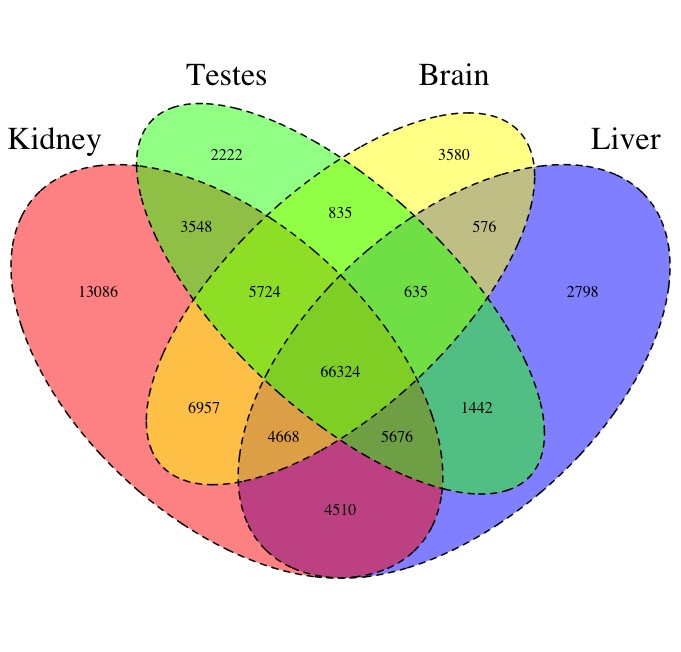
\includegraphics[width=15.0\baselineskip]{/Users/macmanes/Documents/pero_transcriptome/venn.jpeg}}
\begin{quote}
\small{Figure 1. The Venn Diagram.}
\end{quote}   

We then estimated gene expression on each of these tissue-specific datasets, which allowed us to understand expression patterns in the multiple tissues. Specifically, we constructed a Venn diagram ({\hypertarget{Figure 1}{Figure 1}}) that allowed us to visualize the proportion of genes whose expression was limited to a single tissue and those whose expression was ubiquitous. 66324 transcripts are expressed on all tissue types, while 13086 are uniquely expressed in the kidney, 2222 in the testes, 3580 in the brain, and 2798 in the liver. The kidney appears to an outlier in the number of unique sequences, though this could be the result of the recovery of more lowly expressed transcripts that may be the result of deeper sequencing.  \\

In addition to this, we estimated mean TMP (number of transcripts per million) for all transcripts. {\hypertarget{Table 2}{Table 2}} consists of the 10 genes whose mean TMP was the highest. Several genes in this list are predominately  present in a single tissue type. For instance Transcript\_126459, Albumin is very highly expressed in the liver, but less so in the other tissues. It should be noted, however, that making inference based on uncorrected values for TPM is not warranted. Statistical testing for differential expression was not implemented due to the fact that no replicates are available.  \\  

After expression estimation, the filtered assemblies were concatenated together, and after the removal of redundancy with cd-hit-est, 123,123 putative transcripts remained (to be made available on Genbank). From this filtered concatenated dataset, we extracted 71626 putative coding sequences (72Mb, to be made available on Dryad). Of these 71626 sequences, 38221 were complete exons (containing both start and stop codons), while the others were either truncated at the 5-prime end (20239 sequences), the 3-prime end (6445 sequences), or were internal (6721 sequencing with neither stop nor start codon). The results of a Pfam search conducted on the predicted amino acid sequences will be found on Dryad. \\

\textbf{\hypertarget{Table 2}{Table 2}} \\
\begin{center}
\begin{adjustwidth}{-.05in}{-.05in}% adjust the L and R margins by 1 inch
\begin{tabular}{ l l l l l l l}
\textbf{Transcript ID}	&	\textbf{Testes}	&	\textbf{Liver}	&	\textbf{Kidney}	&	\textbf{Brain}	&	\textbf{Genbank ID}	&	\textbf{Gene ID}	\\
\hline
Transcript\_83842	&	2.05E+03	&	6.40E+03	&	1.03E+04	&	5.47E+03	&	DQ073446.1	&	COX2	\\
Transcript\_126459	&	1.43E+01	&	2.22E+04	&	2.77E+01	&	6.73E+00	&	XM\_006991665.1	&	Alb	\\
Transcript\_128937	&	4.39E+00	&	1.91E+04	&	4.74E+02	&	2.23E+00	&	XM\_007627625.1	&	Apoa2	\\
Transcript\_81233	&	1.71E+03	&	5.23E+03	&	6.11E+03	&	3.08E+03	&	XM\_006993867.1	&	Fth1	\\
Transcript\_94125	&	3.67E+01	&	1.08E+04	&	2.09E+03	&	2.75E+00	&	XM\_006977178.1	&	CytP450	\\
Transcript\_119945	&	5.03E+03	&	1.15E+03	&	1.33E+03	&	3.71E+03	&	XM\_008686011.1	&	Ubb	\\
Transcript\_5977	&	4.95E+00	&	1.01E+04	&	3.05E+02	&	3.58E+02	&	XM\_006978668.1	&	Tf	\\
Transcript\_4057	&	2.62E+01	&	9.32E+03	&	1.34E+02	&	8.38E+01	&	XM\_006994871.1	&	Apoc1	\\
Transcript\_112523	&	4.07E+02	&	7.36E+03	&	7.78E+02	&	9.54E+02	&	XM\_006994872.1	&	Apoe	\\
Transcript\_98376	&	1.98E+00	&	8.66E+03	&	1.02E+00	&	2.68E+00	&	XM\_006970208.1	&	Ttr	\\
\end{tabular}
\end{center}
\begin{quote}
\small{Table 2. The 10 transcripts with the highest mean TPM (transcripts per million).}
\end{quote}  
\end{adjustwidth}


\subsection*{Population Genomics}

As detailed above, RNAseq data from 15 individuals were mapped to the reference transcriptome with the resulting BAM files being used as input to the software package ANGSD. The Tajima's D statistic was calculated for all  transcripts covered by at least 14 of the 15 individuals. In brief, a negative Tajima's D - a result of lower than expected average heterozygosity - is often associated with purifying or directional selection, recent selective sweep or population bottleneck. In contrast, a positive value for Tajima's D represents higher than expected average heterozygosity, often associated with balancing selection. \\ 


The distribution of the estimates of Tajima's D for all of the assembled transcripts is shown in Figure 2. The distribution is skewed toward negative values (mean=-0.89, variance=0.58), which is likely the result of purifying selection, a model of evolution commonly invoked for coding DNA sequences \cite{Chamary:2006db}. \hyperlink{Table 3}{Table 3} presents the 10 transcripts whose estimate of Tajima's D is the greatest, while \hyperlink{Table 4}{Table 4} presents the 10 transcripts whose estimate of Tajima's D is the least. The former list of genes is likely to contain transcripts experiencing balancing selection in the studied population. This list includes, interestingly, genes obviously related to solute and water balance (e.g. Clcnkb and a transmembrane protein gene) and immune function (a interferon-inducible GTPase and a Class 1 MHC gene). The latter group, containing transcripts whose estimates of Tajima's D are the smallest are likely experiencing purifying selection. Many of these transcripts are involved in core regulatory functions where mutation may have strongly negative fitness consequences. \\

\vspace{10mm}

\textbf{\hypertarget{Figure 2}{Figure 2}} \\
\centerline{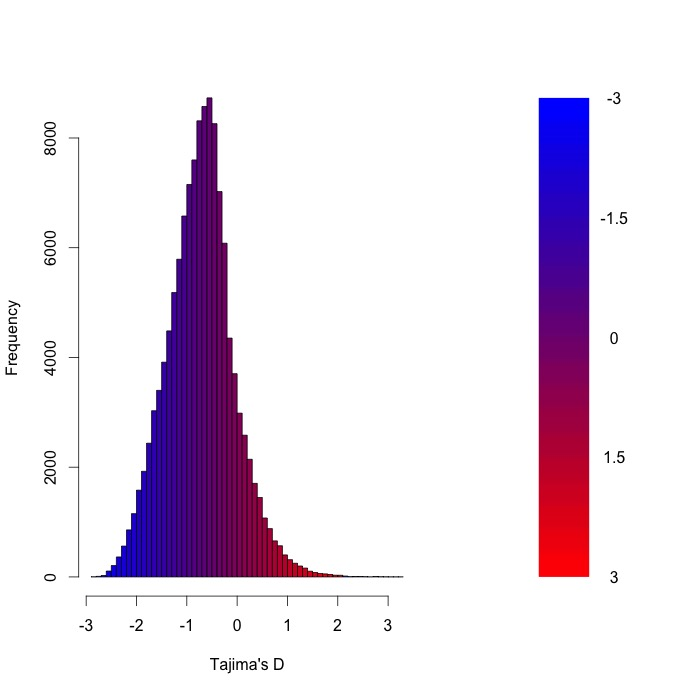
\includegraphics[width=18.0\baselineskip]{/Users/macmanes/Documents/pero_transcriptome/tajD.jpeg}}
\begin{quote}
\small{Figure 2. The distribution of Tajima's D for all putative transcripts.}
\end{quote}  
\vspace{10mm}
\textbf{\hypertarget{Table 3}{Table 3}} \\
\begin{center}
\begin{adjustwidth}{-.75in}{-.75in}% adjust the L and R margins by 1 inch
\begin{tabular}{ l l l l }
\textbf{Transcript ID} & \textbf{GenBank ID} & \textbf{Description} & \textbf{Tajima's D}\\
\hline
Transcript\_49049 & XM\_006533884.1 & heterogeneous nuclear ribonucleoprotein H1 (Hnrnph1) & 3.26\\
Transcript\_38378 & XM\_006522973.1 & Son DNA binding protein (Son) & 3.19\\
Transcript\_126187 & NM\_133739.2 & transmembrane protein 123 (Tmem123) & 3.02\\
Transcript\_70953 & XM\_006539066.1 & chloride channel Kb (Clcnkb) & 2.96 \\
Transcript\_37736 & XM\_006997718.1 & h-2 class I histocompatibility antigen & 2.92 \\
Transcript\_21448 & XM\_006986148.1 & zinc finger protein 624-like & 2.84\\
Transcript\_47450 & NM\_009560.2 zinc & finger protein 60 (Zfp60) & 2.82\\
Transcript\_122250 & XM\_006539068.1 & chloride channel Kb (Clcnkb) & 2.81\\
Transcript\_78367 & XM\_006496814.1 & CDC42 binding protein kinase alpha (Cdc42bpa) & 2.78 \\
Transcript\_96470 & XM\_006987129.1 & interferon-inducible GTPase 1-like & 2.77 \\
 \end{tabular}
\begin{quote}
\small{Table 3. The 10 transcripts with the highest values for Tajima's D, which suggests balancing selection.}
\end{quote}  
\end{adjustwidth}
\end{center}
\vspace{10mm}
\textbf{\hypertarget{Table 4}{Table 4}} \\
\begin{center}
\begin{adjustwidth}{-.75in}{-.75in}% adjust the L and R margins by 1 inch
\begin{tabular}{ l l l l }
\textbf{Transcript ID} & \textbf{GenBank ID} & \textbf{Description} & \textbf{Tajima's D} \\
\hline
Transcript\_84359 & XM\_006991127.1 & nuclear receptor coactivator 3 (Ncoa3) & -2.82\\
Transcript\_87121 & XM\_006970128.1 & methyl-CpG binding domain protein 2 (Mbd2) & -2.82 \\
Transcript\_125755 & EU053203.1 & alpha globin gene cluster & -2.78\\
Transcript\_87128 & XM\_006976644.1 & membrane-associated ring finger (March5) & -2.76 \\
Transcript\_55468 & XM\_006978377.1 & Vpr binding protein (Vprbp) & -2.75\\
Transcript\_116042 & XM\_006980811.1 & membrane associated guanylate kinase (Magi3) & -2.75  \\
Transcript\_18966 & XM\_006982814.1 & ubiquitin protein ligase E3 component n-recognin 5 (Ubr5) & -2.75 \\
Transcript\_122204 & XM\_008772511.1 & zinc finger protein 612 (Zfp612) & -2.75 \\
Transcript\_100550 & XM\_006971297.1 & bromodomain adjacent to zinc finger domain, 1B (Baz1b) & -2.74\\
Transcript\_33267 & XM\_006975561.1 & pumilio RNA-binding family member 1 (Pum1) & -2.75\\
 \end{tabular}
\begin{quote}
\small{Table 4. The 10 transcripts with the lowest values for Tajima's D, which suggests purifying or directional selection.}
\end{quote}  
\end{adjustwidth}
\end{center}

\subsection*{Natural Selection}

To begin to test the hypothesis that selection on transcripts related to osmoregulation is enhanced in the desert adapted \peer, we implemented the branch-site test as described above by setting the sequence corresponding to \peer\:for both Slc2a9 and Vdr as the foreground lineages in 2 distinct program executions. These two transcripts were chosen specifically because they - the former significantly - were recently linked to osmoregulation in a desert rodent \cite{Marra:2014de}. The test for Slc2a9 was highly significant (2$\Delta$Lnl=51.4, df=1, p=0), indicating enhanced selection in \peer\: relative to the other lineages. The branch site test for positive selection conducted on the Vdr gene was non-significant (2$\Delta$Lnl=0.68, df=1, p=1). This limited analysis of selection is to be followed up by an analysis of genome wide patterns of natural selection. \\


\section*{Conclusions}

As a direct result of intense heat and aridity, deserts are thought to be amongst the harshest environments, particularly for mammalian inhabitants. Given that osmoregulation can be challenging for these animals - with failure resulting in death - strong selection should be observed on genes related to the maintenance of water and solute balance. This study aimed to characterize the transcriptome of a desert-adapted rodent species, \peer. Specifically, we characterized the transcriptome of four tissue types (liver, kidney, brain, and testes) from a single individual and supplemented this with population-level renal transcriptome sequencing from 15 additional animals. We identified a set of transcripts undergoing both purifying and balancing selection based on Tajima's D. In addition, we used a branch site test to identify a transcript, likely related to desert osmoregulation, undergoing enhanced selection in \peer\: relative to a set of non-desert rodents.  \\




% Do NOT remove this, even if you are not including acknowledgments
\section*{Acknowledgments}

%MDM would like to acknowledge the support of his wife and children. This work was significantly improved by comments received on a version of the manuscript posted on biorxiv and more generally by supporters of the Open Access and Science movements. 

%\section*{References}
% The bibtex filename
\bibliography{/Users/macmanes/Documents/pero_transcriptome/biblio.bib}








































\end{document}

